% -----------------------------*- LaTeX -*------------------------------
\documentclass[11pt]{report}
\usepackage{scribe_ds603}
\begin{document}


\scribe{Rishabh RP}		% required
\lecturenumber{15}			% required, must be a number
\lecturedate{22/10/2025}		% required, omit year

\maketitle

% ----------------------------------------------------------------------


\section{Evolution of Physical Adverserial Examples}

\subsection{Expectation over Transformations}

\textbf{Motivation: }instead of finding a perturbation that only fools one fixed image, EOT finds a perturbation that on average fools a classifier after the image undergoes the kinds of real-world changes it will see (rotations, scaling, blur). A common EOT-style objective (targeted case) is
% --- EOT objective and practical form (LaTeX snippet) ---
\begin{equation}\label{eq:eot-population}
\min_{\delta\in\mathbb{R}^d}\; 
\mathbb{E}_{t\sim\mathcal{T}}\Big[\ell\big(h_\theta(t(\vec{x}+\vec{\delta})), T\big)\Big]
\;+\; \lambda\, ||\vec{\delta}||_2
\end{equation}

\noindent where \(\vec{x}\) is the clean input, \(\vec{\delta}\) the perturbation, \(\mathcal{T}\) a distribution of transformations (e.g. rotations, translations, blur), \(h_\theta\) the model, and \(\ell\) the loss.

\medskip

\noindent In practice the expectation is approximated by Monte--Carlo sampling (batch size \(B\)):
\begin{equation}\label{eq:eot-mc}
\min_{\delta}\; \frac{1}{B}\sum_{i=1}^B
\ell\big(h_\theta(T_i(\vec{x}+\vec{\delta})), T\big)
\;+\; \lambda\, ||\vec{\delta}||_2, \qquad T_i\overset{\text{iid}}{\sim}\mathcal{T}.
\end{equation}

\noindent The stochastic gradient estimate used by optimizers (e.g. Adam) is
\begin{equation}\label{eq:eot-grad}
\nabla_\delta \mathbb{E}_{t}[\ell(h_\theta(t(\vec{x}+\vec{\delta})),T)]
\approx \frac{1}{B}\sum_{i=1}^B \nabla_\delta \ell\big(h_\theta(T_i(\vec{x}+\vec{\delta})), T\big).
\end{equation}

\begin{figure}[H]
    \centering
    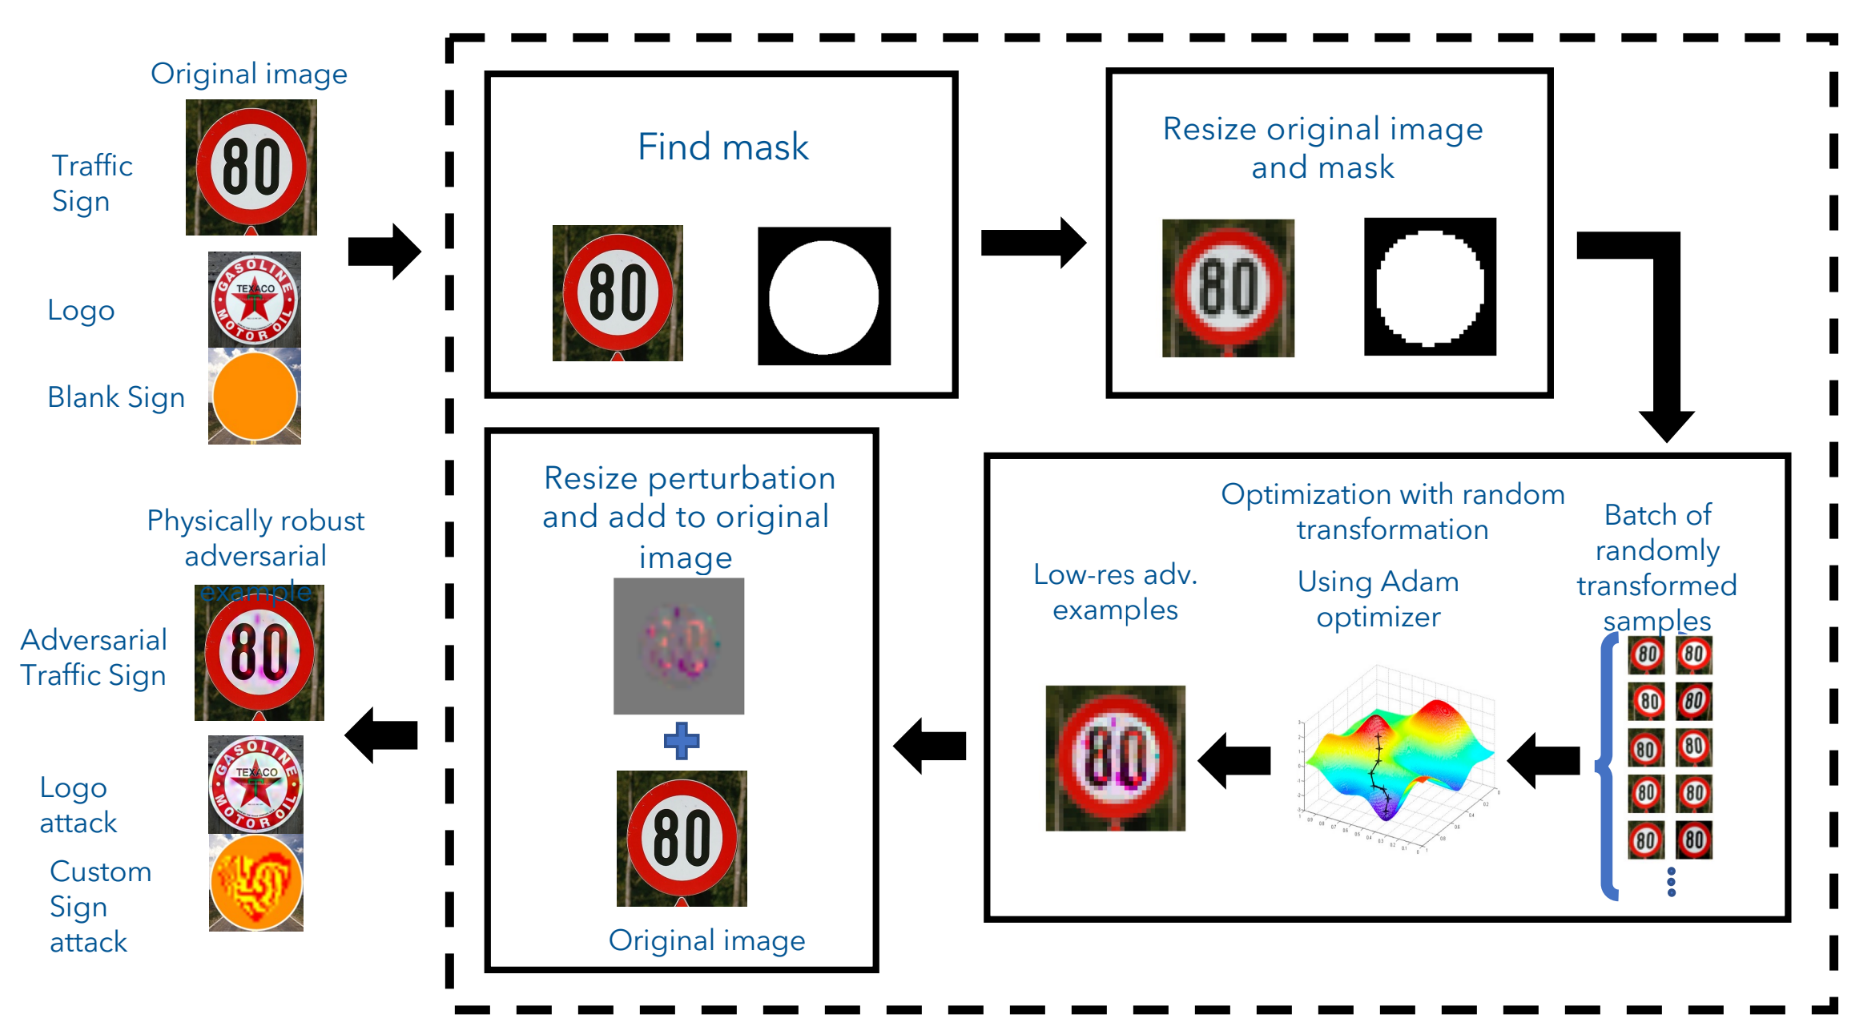
\includegraphics[width=0.5\linewidth]{eot-fig.png}
    \caption{Training of a physically robust adversarial}
    \label{fig:placeholder}
\end{figure}

\subsection{Beyond Vision: Jailbreaks in LLMs}

\begin{enumerate}
    \item Andriushchenko et al.\ demonstrated that simple adaptive attacks (random-search on adversarial suffixes, leveraging log-probs or transfer/prefilling) can reliably jailbreak state-of-the-art safety-aligned LLMs, achieving near 100\% success on many major models. Their attacks are \textbf{highly transferable}: jailbreaks found for one model or via log-prob access frequently transfer to other models (including Claude variants) using transfer or prefilling strategies.

    \item Wei et al. showed that \textbf{competing objectives} occur when a model’s pretraining (language-modelling, instruction-following) objective conflicts with its safety/refusal objective - e.g., the model might follow the user instruction rather than refuse because the user prefix steers it into the instruction-following path.

    \item They also identified \textbf{mismatched generalization}: the safety-fine-tuning distribution does not cover many inputs that the model can handle (via pretraining), so the model fails to generalize its safety behaviour to these ``out-of-safety-training'' but in-capability (pretraining) regions.

    \item Wang et al. show that a weak adversarial policy can beat KataGo (even when it uses search) by exploiting a ``\textbf{pass-attack}'': the adversary stakes a small corner, lets KataGo take most of the board, then triggers a pass sequence, causing KataGo to end the game prematurely with an apparent favorable board but lower actual scoring under Tromp-Taylor rules.
\end{enumerate}

\section{State of Defenses}

\begin{enumerate}
    \item \textbf{Detection of Adversarial Samples:} attempt to distinguish adversarial inputs from clean ones at test time (usually via statistical or model-based anomaly signals), but such detectors often fail under adaptive attacks.
    \item \textbf{Sanitizing via Transformations:} apply randomized / non-differentiable transforms to the input (e.g.\ resize, JPEG, bit-depth reduction) to remove adversarial signal, though EOT shows attackers can explicitly optimize through this distribution.
    \item \textbf{Empirical Adversarial Training:} train on adversarial examples (usually PGD-style) to make the model robust in practice, but robustness is limited to the threat models seen during training and often ``overfits'' to the specific attack recipe.
    \item \textbf{Provable Adversarial Training:} learn with certification (interval bound propagation, convex relaxation, etc.) giving provable guarantees within a norm ball, though current methods are expensive and scale poorly to large models and complex domains.
\end{enumerate}

\subsection{Detection}

One natural approach is to reduce this to a \emph{two-sample testing} problem: given a collection of benign samples $P$ and a collection of (possibly) adversarial samples $Q$, can we test whether $P=Q$?  Maximum Mean Discrepancy (MMD) introduced by Gretton et al. is a classical non–parametric statistic for this.

\medskip
\noindent The population definition is:
\begin{equation}
    \mathrm{MMD}(P,Q,\mathcal{F})
    \;:=\;
    \sup_{f\in\mathcal{F}} \Big( \mathbb{E}_{\vec{x}\sim P}[f(\vec{x})] - \mathbb{E}_{\vec{y}\sim Q}[f(\vec{y})] \Big).
\end{equation}

\noindent $\mathcal{F}$ is a set of functions, which should ideally be expressive enough to be able to distinguish between different distributions. In practice we instantiate $\mathcal{F}$ as the unit ball of a Reproducing Kernel Hilbert Space (RKHS) with kernel $k(\cdot,\cdot)$, which yields the closed–form (kernel) MMD.  Given empirical samples $\{\vec{x}_i\}_{i=1}^n\sim P$ and $\{\vec{y}_j\}_{j=1}^m\sim Q$, we replace expectations by empirical averages and obtain:
\begin{align}
    \mathrm{MMD}_b^2(P_n,Q_m,k)
    \;:=\;
    &\frac{1}{n^2}\sum_{i=1}^n \sum_{i'=1}^n k(\vec{x}_i,\vec{x}_{i'})
    \;+\;
    \frac{1}{m^2}\sum_{j=1}^m \sum_{j'=1}^m k(\vec{y}_j,\vec{y}_{j'})
    \nonumber\\
    &\qquad\qquad
    -\;
    \frac{2}{nm}\sum_{i=1}^n \sum_{j=1}^m k(\vec{x}_i,\vec{y}_j).
\end{align}

\medskip

\noindent The way in which testing is performed is the following:
\begin{enumerate}
    \item Formulate null hypothesis $\mathcal{H}_0: P = Q$ and alternative hypothesis $\mathcal{A}: P \neq Q$
    \item Compare test statistic $\mathrm{MMD}_b^2(P_n,Q_m,k)$ to threshold
    \item Reject the null hypothesis if the statistic exceeds the threshold
\end{enumerate}

\medskip

\noindent However this only looks at adversarial samples as a whole, can we find them one sample at a time? One attempt to do this is to add a new class to our classifier which represents an adversarial example. This is just an \emph{augmented classifier}.

\subsection*{Failure of Adversarial Detection}

\paragraph{Carlini and Wagner (2017).}
Carlini and Wagner showed that attacks can be made arbitrarily stronger simply by increasing the number of optimization iterations.  In particular, they break the MMD-based detector by using their minimum-norm C\&W attack (with thousands of iterations), obtaining adversarial examples that remain undetected even when the detector uses as many as $10{,}000$ samples.

\smallskip
\noindent
They further argue that most defense evaluations fail because they assume the attacker does \emph{not} adapt to the defense.  Instead, one should always construct \emph{adaptive attacks} against the \emph{augmented adversarially-aware classifier}.  They study both \emph{untargeted} attacks (which force the adversarial example to avoid both the original class and the detection rejection class), and \emph{targeted} attacks (which push the example into a specific target class).

\subsection{Data Sanitization}

Can we apply a transformation to the inputs that removes the adversarial noise while preserving the image semantics? Or a bit more mathematically, instead of $h(\vec{x}_{adv})$, we use $h(g(\vec{x}_{adv}))$, where the aim is for $g(\vec{x}_{adv}) \approx \vec{x}$, so that standard classification is performed on transformed input.

\paragraph{TV minimization.}
The objective
\[
\min_{\vec{x}'} \;\;\|(1-B)\odot(\vec{x}'-\vec{x})\|_2 \;+\; \mathrm{TV}_\rho(\vec{x}')
\]
says: on pixels where $B=1$ we are ``allowed'' to change the image (these are the editable pixels), and on pixels where $B=0$ we want $\vec{x}'=\vec{x}$; the first term penalizes deviation on the non-editable region.

\medskip
\noindent
The second term is total variation:
\[
\mathrm{TV}_p(\vec{x}')
=
\sum_{k=1}^K
\Bigg[
\sum_{i=2}^N\big\|\vec{x}'(i,:,k)-\vec{x}'(i-1,:,k)\big\|_\rho
\;+\;
\sum_{j=2}^N\big\|\vec{x}'(:,j,k)-\vec{x}'(:,j-1,k)\big\|_\rho
\Bigg],
\]
i.e.\ we sum horizontal and vertical finite differences of $x'$ (per-channel $k$, where each channel in an image context can be the RGB values), and encourage these differences to be \emph{small}.
TV therefore prefers perturbations that are ``smooth'' or ``piecewise-constant'' (not high-frequency noise), so the optimized $x'$ will not contain spiky pixel-wise noise but will look like a spatially coherent pattern.

\paragraph{Bit Depth Reduction.} Bit-depth reduction maps each pixel channel $\vec{x}_{ijk}\in[0,255]$ to a smaller discrete set of values by reducing the number of bits per channel (e.g.\ from $8$ bits to $3$ bits).  This quantization coarsens the representation and removes fine‐grained high‐frequency perturbations that adversarial examples often rely on.

\subsection*{Failure of Data Sanitization}

\paragraph{Carlini \& Wagner (2018).}
Let \(x\) be the clean input, \(g(\cdot)\) a sanitiser (e.g.\ JPEG, bit-depth reduction, denoiser) and \(h(\cdot)\) the classifier (or classifier+detector).  Defences that apply \(g\) at test time attempt to remove adversarial signal by returning \(g(x)\approx x\).  C\&W observed two key facts used to break such defences.

\begin{enumerate}
  \item \textbf{Adaptive objective.}  An attacker optimizes directly against the \emph{augmented} pipeline:
  \[
    \min_{\delta}\; \|\delta\|_p \quad\text{s.t.}\quad h\big(g(x+\delta)\big)=T \quad\text{(or large loss)}.
  \]
  In practice this is written as an unconstrained problem
  \[
    \min_{\delta}\; \|\delta\|_p + c\cdot \ell\big(h(g(x+\delta)),T\big),
  \]
  and solved by iterative optimization (C\&W use many iterations).
  \item \textbf{Gradient approximation / straight-through.} If \(g(x)\approx x\) then the backward signal through \(g\) is small or ill-behaved; C\&W and later works therefore (i) use a differentiable surrogate for \(g\), (ii) use a straight-through estimator (treat \(g\) as identity in the backward pass), or (iii) approximate
  \[
    \nabla_\delta \ell\big(h(g(x+\delta)),y\big)
    \approx
    \nabla_\delta \ell\big(h(x+\delta),y\big)
  \]
  when \(g\) is nearly identity.  Any of these yield usable gradients and enable the optimizer to converge to very small-norm perturbations that survive \(g\).
\end{enumerate}

\noindent\textbf{Net effect:} since \(g\) must preserve clean accuracy it cannot be a violent mapping away from \(x\); this ``near-identity'' property makes it possible to (a) approximately backpropagate through the sanitizer, (b) use iterative minimum-norm methods (C\&W) for thousands of steps, and (c) produce adversarial examples that both fool \(h\) \emph{and} pass the sanitizer — thereby breaking detection/sanitization defences.


\section{Empirical Adversarial Training (Madry et al., 2017)}

\paragraph{Minimax objective.}
Empirical adversarial training frames robustness as a minimax problem:
\begin{equation}\label{eq:adv-train}
h_{robust} = \text{argmin}_{h}\; \mathbb{E}_{(\vec{x},y)\sim\mathbb{\hat{P}}_n}\Big[ \; \max_{\|\delta\| \le \epsilon} \; L_\text{proxy}\big((\vec{x}+\vec{\delta}, y),h\big) \;\Big],
\end{equation}
where the inner maximization seeks the worst-case perturbation \(\vec{\delta}\) (within an \(\ell_p\) ball of radius \(\epsilon\)) and the outer minimization trains model parameters to minimize this worst-case loss.

\noindent Rewriting this, we want to solve $\min_{\vec{\theta}} \  \max_{\vec{\delta} \in N} \ L(\vec{\theta},\vec{x}+\vec{\delta},y) = \min_{\vec{\theta}} \  \max_{\vec{\delta} \in N} \  g(\vec{\theta}, \vec{\delta})$. We want to be able to perform descent in $\vec{\theta}$.

\paragraph{Approximation in practice.}
Since the inner maximization is intractable exactly, Madry et al.\ approximate it by multi-step Projected Gradient Descent (PGD):
\[
\delta^{(t+1)} \leftarrow \Pi_{\|\delta\|\le\epsilon}\big(\delta^{(t)} + \alpha\,\mathrm{sign}(\nabla_\delta \ell(h_\theta(x+\delta^{(t)}),y))\big)
\]
(or the full gradient step for \(\ell_2\)), run for \(K\) iterations to produce a high-loss adversarial example used for training.
\begin{theorem}\label{Danskin}
\textbf{Danskin's Theorem}: Let $N$ be non-empty and compact, and $g(\cdot,\vec{\delta})$ be differentiable for every $\vec{\delta} \in N$ and $\triangledown_{\vec{\theta}} \ g(\vec{\theta}, \vec{\delta})$ is continuous. Then, the max function
\[
    f(\vec{\theta}) = \max_{\vec{\delta} \in N} \  g(\vec{\theta}, \vec{\delta})
\]

\noindent is locally Lipschitz continuous, and if $\vec{\delta}_{\vec{\theta}}^*$ is a unique maximizer, then 
\[
     \triangledown f(\vec{\theta}) = \triangledown_{\vec\theta} \ g(\vec{\theta}, \vec{\delta}_{\vec{\theta}}^*)
\]
\end{theorem}

\begin{corollary}
If $\vec{\delta^*} \in N$ and is a maximiser for
$\max_{\vec{\delta}} \ L(\vec{\theta}, \vec{x}+\vec{\delta}, y)$
, then
$-\triangledown_{\vec{\theta}} \  L(\vec{\theta}, \vec{x}+\vec{\delta^*}, y)$ is a descent direction for $f(\vec{\theta})$
\end{corollary}

\noindent Danskin's theorem gives us a way to approximate gradient descent for our minimax objective. We can find an approximation for the inner maximization through gradient ascent, and then differentiate our loss function at the maximiser, to perform descent for the outer function to find $\vec{\theta}$. 

\begin{algorithm2e}[H]
\DontPrintSemicolon
\SetKwInOut{giv}{Given}
\SetKwInOut{out}{Output}
\giv{epochs $E$, dataset $\{(x_i,y_i)\}_{i=1}^N$, step size $\alpha$}
\For{$e = 1,2,\dots,E$}{
    \For{$i = 1,2,\dots,N$}{
        1. compute adversarial example $x^{T}_{i,\mathrm{adv}}$ for current state $\theta_{t-1}$\;
        2. compute adversarial loss $L(h_{\theta_{t-1}}(x^{T}_{i,\mathrm{adv}}), y)$\;
        3. compute gradient $\nabla_{\theta}L(h_{\theta_{t-1}}(x^{T}_{i,\mathrm{adv}}), y)$\;
        4. update parameters $\theta_t \leftarrow \theta_{t-1} - \alpha\,\nabla_{\theta}L(h_{\theta_{t-1}}(x^{T}_{i,\mathrm{adv}}), y)$\;
    }
}
\out{$\theta_E$}
\caption{Empirical Adversarial Training (Madry et al.)}
\label{alg:madry_pgd}
\end{algorithm2e}

\paragraph{Pros}
\begin{itemize}
    \item simple to implement
    \item works in practice against the same adversaries it trains on
    \item resistant to adaptive attacks (when attacks match the training threat model)
    \item no gradient obfuscation (the gradients are explicit)
\end{itemize}

\paragraph{Cons}
\begin{itemize}
    \item computationally expensive; adds significant training time
    \item does not generalize across adversaries (norms / threat models)
    \item not provably robust
\end{itemize}

\section*{Bibliography}

\begin{enumerate}

\item Anish Athalye, Logan Engstrom, Andrew Ilyas, and Kevin Kwok.
Synthesizing robust adversarial examples via expectation over transformations.
2017.

\item  Maksym Andriushchenko, Francesco Croce, Nicolas Flammarion
Jailbreaking Leading Safety-Aligned LLMs with Simple Adaptive Attacks
2024.

\item Alexander Wei, Nika Haghtalab, Jacob Steinhardt
Jailbroken: How Does LLM Safety Training Fail?
2023.

\item Tony T. Wang, Adam Gleave, Tom Tseng, Kellin Pelrine, Nora Belrose, Joseph Miller, Michael D. Dennis, Yawen Duan, Viktor Pogrebniak, Sergey Levine, Stuart Russell
Adversarial Policies Beat Superhuman Go AIs
ICML 2023.

\item Arthur Gretton, Karsten Borgwardt, Malte Rasch, Bernhard Schölkopf, and Alexander Smola.
A Kernel Two-sample Test.
Journal of Machine Learning Research 13: 723-773, 2012.

\item Nicholas Carlini and David Wagner.
Towards Evaluating the Robustness of Neural Networks.
IEEE Symposium on Security and Privacy (S&P), 2017.

\item Nicholas Carlini and David Wagner.
Adversarial Examples are Not Easily Detected: Bypassing Ten Detection Methods.
ICML 2017 Workshop, and later updated ICML 2018.

\item Aleksander Madry, Aleksandar Makelov, Ludwig Schmidt, Dimitris Tsipras, and Adrian Vladu.
Towards Deep Learning Models Resistant to Adversarial A
ttacks.
ICLR 2018.

\end{enumerate}

\end{document}

